% ---------------------------------------------------------
% Project: PhD KAPPA
% File: results.5.tex
% Author: Andrea Discacciati
%
% Purpose: Paper V (results)
% ---------------------------------------------------------

\section{Paper V}

The aim of \citetalias{discacciati_goodness_2015} was to present, discuss, and practically illustrate 3 tools that can help to evaluate the goodness of fit of a dose--response meta-analysis: deviance, coefficient of determination ($R^2$), and \rveplot.

These tools were presented in  \citetalias{discacciati_goodness_2015} using the notation following the `one-stage' or `pool-first' dose--response meta-analytic approach. However, they can be equivalently expressed in terms of notation based on the two-stage approach.  In the next sections, we will follow this alternative way of presenting the 3 tools. Note that in the following exposition it is assumed that $\boldsymbol{\Sigma}_i = \mathbf{V}(\boldsymbol{\beta}_i)$ and that the assigned dose $x_{i0}$ for the referent level of the exposure  is equal to 0 for all the studies.

\subsection{Goodness of fit tools for dose--response meta-analysis}
\subsubsection{Deviance}

In dose--response meta-analysis, the data points to be fitted are the non-referent logRRs reported by the single studies. Therefore, analysis of  residuals can be useful to evaluate how close reported and predicted logRRs are at each exposure level. Study-specific vectors of residuals, calculated as the difference between the observed logRRs and the model predictions from the overall dose--response function, are equal to
\begin{equation*}
\mathbf{e}_i = \mathbf{y}_i - \mathbf{X}_i \mathbf{Z}_i \hat{\boldsymbol{\theta}}.
\end{equation*}

A statistic for the absolute goodness of fit based on these residuals is the deviance statistic, which is defined as
\begin{equation}
D = \sum_{i=1}^{K} D_i = \sum_{i=1}^{K} \left(\mathbf{y}_i - \mathbf{X}_i \mathbf{Z}_i \hat{\boldsymbol{\theta}}\right)^\top \mathbf{S}_i^{-1} \left(\mathbf{y}_i - \mathbf{X}_i \mathbf{Z}_i \hat{\boldsymbol{\theta}}\right) = \sum_{i=1}^{K} \mathbf{e}_i^\top \mathbf{S}_i^{-1} \mathbf{e}_i.
\label{eq:deviance}
\end{equation}

The deviance measures the total absolute distance between reported and fitted logRRs  while taking into account the correlation structure of the study-specific logRRs through the matrices $\mathbf{S}_i$ --- that is, the generalized residual sum of squares (GRSS). Intuitively, the smaller the deviation, the closer the reported and predicted logRRs will be.

Building on the assumption that the single logRRs are normally distributed, the deviance provides a test for model specification. Under the null hypothesis that the model is correctly specified, $D$ is asymptotically distributed as a chi-square random variable  with $n-qm$ degrees of freedom (df), where $n = \sum_{i=1}^K J_i$. This means that testing for model specification amounts to testing whether, under the null hypothesis, the residual variance corrected for the correlation between the logRRs is larger than one would expect. A small $p$-value indicates that there is evidence that the posited model fails in accounting for the observed variation among the logRRs.

\subsubsection{Coefficient of determination}

A descriptive statistic that can be used as a complement to the deviance to summarize the goodness of fit of a given model is the coefficient of determination ($R^2$). This statistic evaluates the agreement between observed and predicted logRRs and, unlike the deviance, is bounded between 0 and 1 \citep{hagquist_goodness_1998, kvalseth_cautionary_1985}.

Given that the generalized total sum of squares (GTSS) is equal to $\sum_{i=1}^{K} \mathbf{y}_i^\top \mathbf{S}_i^{-1} \mathbf{y}_i$, and given the lack of the intercept term, $R^2$ is defined, following the work of \citet[section~6.2]{theil_economic_1961} and \citet{buse_goodness_1973}, as:
\begin{equation*}
R^2 = 1-\frac{\textrm{GRSS}}{\textrm{GTSS}} = 1 - \frac{\sum\limits_{i=1}^{K} \left(\mathbf{y}_i - \mathbf{X}_i \mathbf{Z}_i \hat{\boldsymbol{\theta}}\right)^\top \mathbf{S}_i^{-1} \left(\mathbf{y}_i - \mathbf{X}_i \mathbf{Z}_i \hat{\boldsymbol{\theta}}\right)}{\sum\limits_{i=1}^{K} \mathbf{y}_i^\top \mathbf{S}_i^{-1} \mathbf{y}_i}.
\end{equation*}

$R^2$ is a dimensionless index that measures the proportion of the GTSS accounted for by the exposure and study-level covariates. It takes value 0 if the dose--response meta-analytic model explains no variability in the observed logRRs, while it takes value 1 if the model accounts for all the observed variability among the logRRs. Generally, a low $R^2$ might be an indication that a more flexible transformation of the exposure and/or  a meta-regression model is needed.

An adjusted version of $R^2$ that is penalized by the number of total covariates included in the first and second stage of the dose--response meta-analysis is given by
\begin{equation*}
R_{\textrm{adj}}^2 = 1- \frac{n}{n-qm}\left(1-R^2\right).
\end{equation*}

$R_{\textrm{adj}}^2$ increases only if the increment in $R^2$ is larger than what would be expected by chance alone and can prove useful to compare the fit of non-nested models.

\subsubsection{Visual assessment}

Visual inspection of the model fit can reveal important data features and model shortcomings that may otherwise go undetected \citep{kvalseth_cautionary_1985}. Visual assessment of the goodness of fit in dose--response meta-analysis is however made more difficult due to the fact that the study-specific logRRs are correlated. As a consequence, the fitted dose--response curve might not even pass through the data points, depending on the particular correlation structure of the residuals, and a simple plot overlaying the dose--response curve to the reported logRRs might therefore be highly misleading. This issue is illustrated in figure \ref{fig:visual_wrong} using the aggregated data reported in table \ref{table:examplecorr}. This is the reason why, for example, in figure \ref{fig:ss_loc} we decided to not overlay the observed RRs to the study-specific regression curves. To avoid this problem, one can plot the decorrelated residuals versus the exposure. 

\begin{figure}[]
\centering
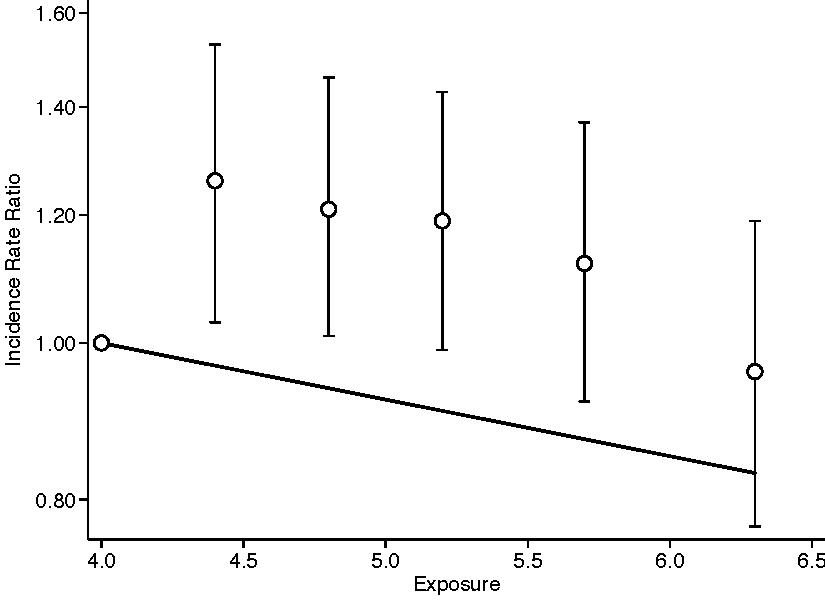
\includegraphics[width=.8\linewidth]{figures/visual_wrong.pdf}
\caption[Plot overlaying one study-specific dose--response curve to the reported IRRs]{Fitted linear trend (solid line) based on IRRs (hollow circles) and exposure values reported in a single study (table \ref{table:examplecorr}). Due to the correlation among the IRRs, the linear trend does not pass through the data points. The vertical axis is on the natural log scale.}
\label{fig:visual_wrong}
\end{figure}

The decorrelated residuals are obtained by decomposing each study-specific matrix $\mathbf{S}_i$ through Cholesky factorization, so that $\mathbf{S}_i=\mathbf{C}_i \mathbf{C}_i^\top$, where $\mathbf{C}_i$ is a lower triangular matrix.\footnote{Equivalently, $\mathbf{S}_i^{-1}=(\mathbf{C}_i^{-1})^\top (\mathbf{C}_i^{-1})$.} The study-specific decorrelated residuals $\mathbf{e}_i^*$ are then obtained by multiplying the inverse of $\mathbf{C}_i$ by the difference between reported and fitted logRRs:
\begin{equation*}
\mathbf{e}_i^* = \mathbf{C}_i^{-1}  \left(\mathbf{y}_i - \mathbf{X}_i \mathbf{Z}_i \hat{\boldsymbol{\theta}}\right) = \mathbf{C}_i^{-1} \mathbf{e}_i.
\end{equation*}

Lastly, the decorrelated residuals for all the studies are plotted against the exposure.

Although the vertical distances from the reference line drawn at $e^*=0$ have no meaningful interpretation, it is still possible to assess how the pooled dose--response curve fits the data according to exposure levels. If the fit is perfect, all the points will lie on the reference line. As the fit gets worse, the points will move away from it. A pattern in the decorrelated residuals might indicate for example that the fit of the model is adequate only at certain exposure levels or that study-level covariates need to be taken into account, therefore suggesting the need of a richer dose--response model. Overlaying a LOWESS smoother to the plot or changing the shape/color of the points according to study-level covariates might help to detect such patterns.


\subsubsection{Goodness of fit of study-specific dose--response models}

The three tools presented so far can be also used to assess the goodness of fit of the first-stage study-specific dose--response models, if one wishes so. Only minor modifications in the formulae are necessary. In particular, it is sufficient to replace the pooled parameter vector $\hat{\boldsymbol{\theta}}$ with the study-specific parameter vectors $\hat{\boldsymbol{\beta}}_i$ and drop the second-stage design matrix $\mathbf{Z}_i$.

Let the study-specific decorrelated residuals be
\begin{equation*}
\tilde{\mathbf{e}}_i^* = \mathbf{C}_i^{-1}  \left(\mathbf{y}_i - \mathbf{X}_i \hat{\boldsymbol{\beta}}_i\right) = \mathbf{C}_i^{-1} \tilde{\mathbf{e}}_i.
\end{equation*}
These residuals can be used to construct study-specific \rveplot s.

The deviance for the $i$-th study-specific dose--response regression model is defined as
\begin{equation*}
\tilde{D}_i = \left(\mathbf{y}_i - \mathbf{X}_i \hat{\boldsymbol{\beta}}_i\right)^\top \mathbf{S}_i^{-1} \left(\mathbf{y}_i - \mathbf{X}_i \hat{\boldsymbol{\beta}}_i\right) = \tilde{\mathbf{e}}_i^\top \mathbf{S}_i^{-1} \tilde{\mathbf{e}}_i,
\end{equation*}
and when the $i$-th study-specific model is correctly specified, $\tilde{D}_i$ asymptotically follows a chi-square random variable with $J_i-q$ degrees of freedom. Moreover, as the $K$ studies are summed to be independent, it is also possible to set up a joint test for model specification of all the $K$ first-stage study-specific dose--response regressions. In fact, under the null hypothesis that all the first-stage models are correctly specified, the sum of the $K$ study-specific deviances $\tilde{D}_i$ is asymptotically distributed as a chi-square random variable with $\sum_{i=1}^K(J_i - q) = n-Kq$ degrees of freedom:
\begin{equation}
\tilde{D} = \sum_{i=1}^K \tilde{D}_i = \sum_{i=1}^{K} \tilde{\mathbf{e}}_i^\top \mathbf{S}_i^{-1} \tilde{\mathbf{e}}_i \sim \chi_{n-Kq}^2.
\label{eq:dtilde}
\end{equation}

Lastly, the coefficient of determination for the $i$-th study is defined as
\begin{equation*}
R_i^2 = 1- \frac{\left(\mathbf{y}_i - \mathbf{X}_i  \hat{\boldsymbol{\beta}}_i\right)^\top \mathbf{S}_i^{-1} \left(\mathbf{y}_i - \mathbf{X}_i  \hat{\boldsymbol{\beta}}_i\right)}{ \mathbf{y}_i^\top \mathbf{S}_i^{-1} \mathbf{y}_i}.
\end{equation*}


\subsubsection{Relation between \textit{D} and  \textit{Q} statistics}

Analogously to the vector of decorrelated residuals $\mathbf{e}_i^*$, let the following objects
\begin{align*}
\mathbf{y}_i^* &= \mathbf{C}_i^{-1}  \mathbf{y}_i \\
\mathbf{X}_i^* &= \mathbf{C}_i^{-1}  \mathbf{X}_i,
\end{align*}
be the vector of decorrelated non-referent logRRs and the decorrelated design matrix for the $i$-th study. Suppose also for sake of simplicity that $\mathbf{Z}_i=\mathbf{I}_{(J_i)}$ for $i=1,\ldots,K$. 

It is possible to show that the difference between $D$ [equation (\ref{eq:deviance})] and $Q$ [equation (\ref{eq:multiq})] is equal to $\tilde{D}$ [equation (\ref{eq:dtilde})]. In fact,
\begin{align*}
%\begin{split}
D &= \sum_{i=1}^{K} \left(\mathbf{y}_i - \mathbf{X}_i \hat{\boldsymbol{\theta}}\right)^\top \mathbf{S}_i^{-1} \left(\mathbf{y}_i - \mathbf{X}_i  \hat{\boldsymbol{\theta}}\right) = \\
&= \sum_{i=1}^{K} \left(\mathbf{y}_i^* - \mathbf{X}_i^* \hat{\boldsymbol{\theta}}\right)^\top \left(\mathbf{y}_i^* - \mathbf{X}_i^*  \hat{\boldsymbol{\theta}}\right) = \\
&=\sum_{i=1}^K \left( \mathbf{y}_i^{*\top} \mathbf{y}_i^{*} - \mathbf{y}_i^{*} \mathbf{X}_i^* \hat{\boldsymbol{\theta}} - \hat{\boldsymbol{\theta}}^\top \mathbf{X}_i^{*\top} \mathbf{y}_i^{*} - \hat{\boldsymbol{\theta}}^\top \mathbf{X}_i^{*\top} \mathbf{X}_i^* \hat{\boldsymbol{\theta}} \right)
%\end{split}
\end{align*}
and
\begin{align*}
%\begin{split}
Q &= \sum_{i=1}^K \left(\hat{\boldsymbol{\beta}}_i - \hat{\boldsymbol{\theta}} \right)^\top  \hat{\mathbf{V}}(\boldsymbol{\beta}_i)^{-1} \left(\hat{\boldsymbol{\beta}}_i - \hat{\boldsymbol{\theta}} \right) = \\
&= \sum_{i=1}^K \left(\hat{\boldsymbol{\beta}}_i - \hat{\boldsymbol{\theta}} \right)^\top \underbrace{\left(\mathbf{X}_i^{\top} \mathbf{S}_i^{-1} \mathbf{X}_i \right)}_{\textrm{GLS estimator}} \left(\hat{\boldsymbol{\beta}}_i - \hat{\boldsymbol{\theta}} \right) = \\
&= \sum_{i=1}^K \left(\hat{\boldsymbol{\beta}}_i - \hat{\boldsymbol{\theta}} \right)^\top \left(\mathbf{X}_i^{*\top} \mathbf{X}_i^* \right) \left(\hat{\boldsymbol{\beta}}_i - \hat{\boldsymbol{\theta}} \right) = \\
&= \sum_{i=1}^K \left( \mathbf{X}_i^* \hat{\boldsymbol{\beta}}_i - \mathbf{X}_i^* \hat{\boldsymbol{\theta}} \right)^\top \left( \mathbf{X}_i^* \hat{\boldsymbol{\beta}}_i - \mathbf{X}_i^* \hat{\boldsymbol{\theta}} \right) = \\
&= \sum_{i=1}^K \left( \mathbf{X}_i^* \left(\mathbf{X}_i^{*\top} \mathbf{X}_i^* \right)^{-1} \mathbf{X}_i^{*\top} \mathbf{y}_i^* - \mathbf{X}_i^* \hat{\boldsymbol{\theta}} \right)^\top \left( \mathbf{X}_i^* \left(\mathbf{X}_i^{*\top} \mathbf{X}_i^* \right)^{-1} \mathbf{X}_i^{*\top} \mathbf{y}_i^* - \mathbf{X}_i^* \hat{\boldsymbol{\theta}} \right) = \\
&=\sum_{i=1}^K \left( \mathbf{H}_i^* \mathbf{y}_i^* - \mathbf{X}_i^* \hat{\boldsymbol{\theta}} \right)^\top \left( \mathbf{H}_i^* \mathbf{y}_i^* - \mathbf{X}_i^* \hat{\boldsymbol{\theta}} \right) = \\
&=\sum_{i=1}^K \left( \mathbf{y}_i^{*\top} \underbrace{\mathbf{H}_i^{*\top} \mathbf{H}_i^{*}}_{\mathclap{\mathbf{H}_i^{*} \textrm{ is idempotent}}} \mathbf{y}_i^{*} - \mathbf{y}_i^{*} {\mathbf{H}_i^{*\top} \mathbf{X}_i^*} \hat{\boldsymbol{\theta}} - \hat{\boldsymbol{\theta}}^\top \underbrace{\mathbf{X}_i^{*\top} \mathbf{H}_i^{*}}_{\mathclap{\mathbf{H}_i^* \textrm{ is symmetric and } \mathbf{H}_i^* \mathbf{X}_i^* = \mathbf{X}_i^*}} \mathbf{y}_i^{*} + \hat{\boldsymbol{\theta}}^\top \mathbf{X}_i^{*\top} \mathbf{X}_i^* \hat{\boldsymbol{\theta}} \right) = \\
&=\sum_{i=1}^K \left( \mathbf{y}_i^{*\top}  \mathbf{H}_i^{*} \mathbf{y}_i^{*} - \mathbf{y}_i^{*} \mathbf{X}_i^* \hat{\boldsymbol{\theta}} - \hat{\boldsymbol{\theta}}^\top \mathbf{X}_i^{*\top} \mathbf{y}_i^{*} + \hat{\boldsymbol{\theta}}^\top \mathbf{X}_i^{*\top} \mathbf{X}_i^* \hat{\boldsymbol{\theta}} \right).
%\end{split}
\end{align*}

The difference between $D$ and $Q$ is therefore
\begin{align*}
%\begin{split}
D-Q &=\sum_{i=1}^K \left( \mathbf{y}_i^{*\top} \mathbf{I}_{(J_i)} \mathbf{y}_i^{*} -  \mathbf{y}_i^{*\top} \mathbf{H}_i^* \mathbf{y}_i^{*} \right) = \\
&=\sum_{i=1}^K \mathbf{y}_i^{*\top}  \underbrace{\left(  \mathbf{I}_{(J_i)} - \mathbf{H}_i^* \right) }_{{\mathclap{\textrm{symmetric and idempotent}}}}  \mathbf{y}_i^{*} = \\
&= \sum_{i=1}^K \mathbf{y}_i^{*\top} \left(  \mathbf{I}_{(J_i)} - \mathbf{H}_i^*  \right)^\top \left(  \mathbf{I}_{(J_i)} - \mathbf{H}_i^*  \right)  \mathbf{y}_i^{*} = \\
&= \sum_{i=1}^K \tilde{\mathbf{e}}_i^{*\top} \tilde{\mathbf{e}}_i^* = \\
&= \sum_{i=1}^K \tilde{\mathbf{e}}_i^\top \left(\mathbf{C}_i^{-1}\right)^\top \left(\mathbf{C}_i^{-1}\right) \tilde{\mathbf{e}}_i = \\
&= \sum_{i=1}^K \tilde{\mathbf{e}}_i^\top \mathbf{S}_i^{-1} \tilde{\mathbf{e}}_i = \tilde{D}.
%\end{split}
\end{align*}

A direct consequence of this relation is that $D \ge Q$. In particular, $D = Q$ when all the first-stage study-specific regression models fit perfectly the reported logRRs --- that is, $R_i^2=1$ for every $i$.

Perhaps not surprisingly at this point, the degrees of freedom of $D$ minus the degrees of freedom of $Q$ is equal to the degrees of freedom of $\tilde{D}$. In fact
\begin{equation*}
n-qm - (Kq - qm) = n-Kq.
\end{equation*} 

\subsection{Goodness of fit assessment: dose--response meta-analysis on body mass index and incidence of localized prostate cancer}
\label{sec:examplegof}

To illustrate the 3 tools introduced in the previous section, we will evaluate the goodness of fit of the updated dose--response meta-analysis on BMI and incidence of localized prostate cancer presented in section \ref{section:results4updated}. This meta-analysis was based on 18 prospective studies for a total of 46 non-referent logRRs.

The identity transformation for BMI --- that is, modeling BMI linearly --- resulted in a particularly poor goodness of fit (model 1). In particular, the test for model specification showed evidence of lack of fit, as indicated by a deviance of 64 on $46-1=45$ degrees of freedom ($p=0.03$) (table \ref{table:gof_table}). The percentage of total variability in the non-referent logRR estimates explained by this model was $R^2=29\%$. Furthermore, the \rveplot{} showed that the fit of the model was poor. In particular, the decorrelated residuals were mostly positive for low values of the rescaled exposure, while they were almost all negative for high exposure values (figure \ref{fig:gof_loc}, panel A). 

The lack of fit of model 1 was addressed by modeling BMI using RCS with 3 knots positioned at the 10th, 50th, and 90th percentiles of the exposure distribution (model 2). The improvement in the goodness of fit of model 2 over model 1 was reflected by the increase in the coefficient of determination (from 29\% to 48\%) and by the large reduction in the deviance with respect to the difference in the degrees of freedom ($D=64-47=17$, $\df=45-44=1$, $p_{\textrm{non-linearity}}<0.001$) (table \ref{table:gof_table}). Furthermore, the \rveplot{} reflected the improved fit of model 2, especially for the right tail of the exposure distribution (figure \ref{fig:gof_loc}, panel B). Lastly, from the test for model specification, we observed no evidence of lack of fit for model 2 ($D=47$, $\df=46-2=44$, $p=0.35$).

\begin{figure}[h]
\centering
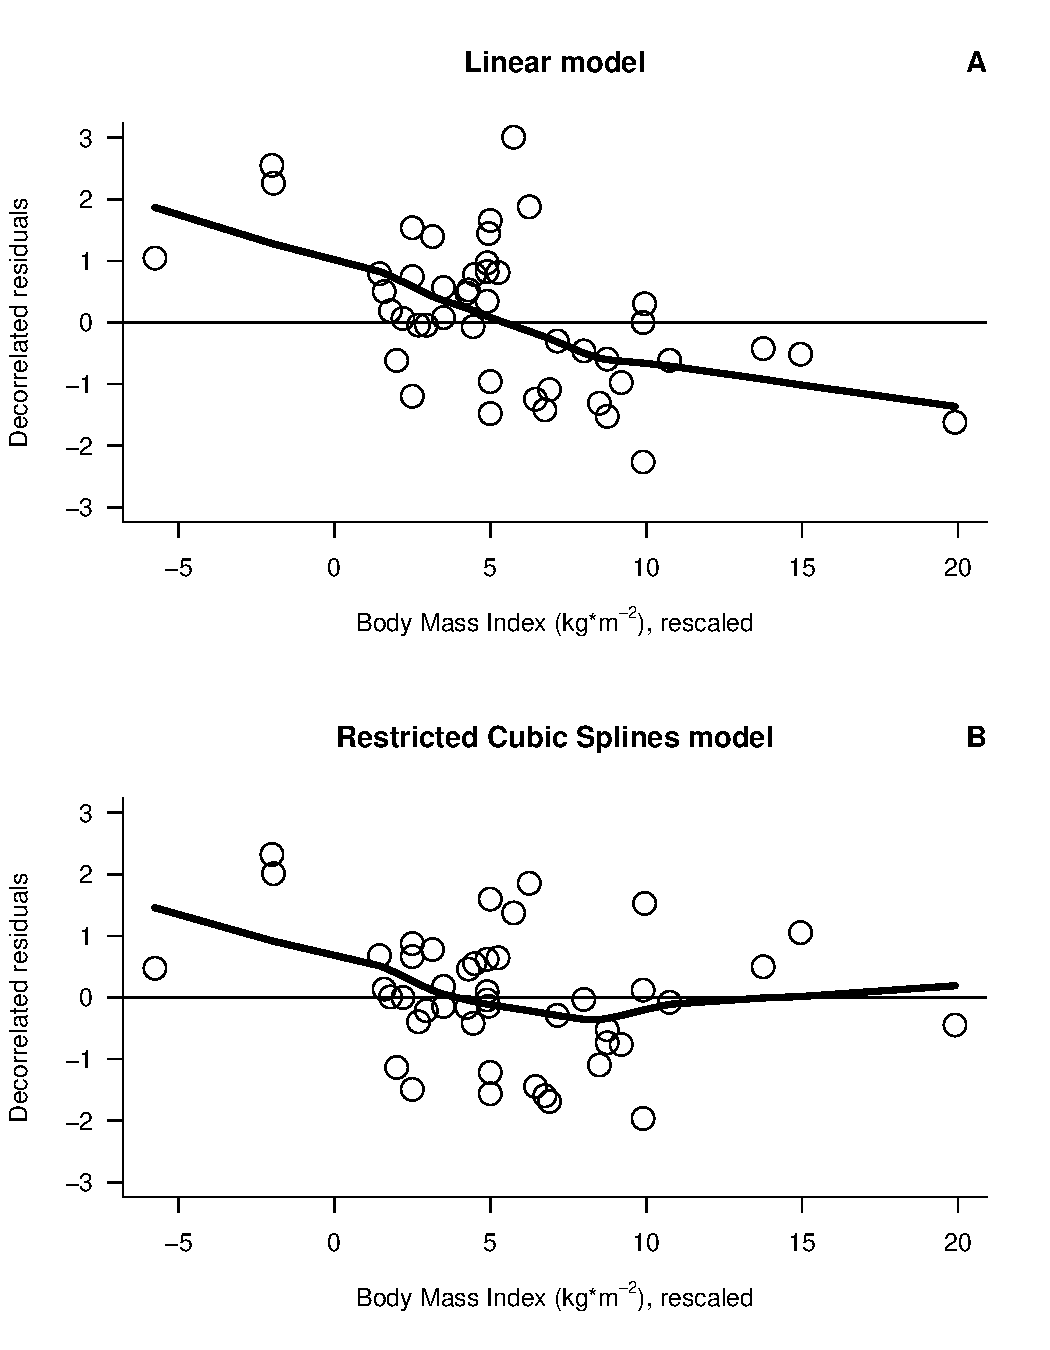
\includegraphics[width=\linewidth]{figures/gof.pdf}
\caption[Decorrelated-residuals--versus--exposure plots for the dose--response meta-analysis on BMI and localized prostate cancer incidence]{Decorrelated residuals (hollow circles) and LOWESS smoother (black line) for model 1 (panel A) and for model 2 (panel B) in the updated dose--response meta-analysis on BMI and incidence of localized prostate cancer presented in section \ref{section:results4updated}.}
\label{fig:gof_loc}
\end{figure}

Similar conclusions regarding the goodness of fit of the pooled dose--response curve following a non-linear transformation of the exposure were reached when using the other two transformations proposed in section \ref{section:results4updated}, namely RCS with 3 knots positioned at the 25th, 50th, and 75th percentiles (model 3), and quadratic polynomial (model 4). A summary of the goodness of fit for the 4 models considered here is reported in table \ref{table:gof_table}.

\bigskip

\begin{table}[hb]
\centering
\caption[Goodness of fit measures for the dose--response meta-analysis on BMI and localized prostate cancer incidence]{Goodness of fit measures for the updated dose--response meta-analysis on BMI and incidence of localized prostate cancer presented in section \ref{section:results4updated}}
\label{table:gof_table}
\begin{threeparttable}
\begin{tabular}{cccccccc}
\hline
\textbf{Model} & \textbf{BMI transformation} & \textbf{Deviance} & \textbf{df} & \textbf{\textit{p}-value}\tnote{a} & \textbf{\textit{p}-value}\tnote{b} & \textbf{$\mathbf{R^2}$} & \textbf{$\mathbf{R_{\textrm{adj}}^2}$} \\ \hline
1        & Linear (identity)                                                          & 64                & 45          & 0.03                      & ---                       & 29\%                    & 29\%                                   \\
2        & RCS with 3 knots\tnote{c}                                                                & 47                & 44          & 0.35                      & $<0.001$                  & 48\%                    & 45\%                                   \\
3        & RCS with 3 knots\tnote{d}                                                                & 44                & 44          & 0.45                      & $<0.001$                  & 50\%                    & 48\%                                   \\
4        & Quadratic polynomial                                                       & 49                & 44          & 0.26                      & $<0.001$                  & 45\%                    & 42\%                                   \\ \hline
\end{tabular}
\begin{tablenotes}
\item [a] \footnotesize $p$-value from the test for model specification.
\item [b] \footnotesize $p$-value for relative goodness of fit with respect to model 1.
\item [c] \footnotesize Knots positioned at the 10th, 50th, and 90th percentiles of BMI distribution.
\item [d] \footnotesize Knots positioned at the 25th, 50th, and 75th percentiles of BMI distribution.  
\end{tablenotes}
\end{threeparttable}
\end{table}





